%%%%%%%%%%%%%%%%%%%%%%%%%%%%%%%%%%%%%%%%%%%%%%
%%%%%%%%%%%% Method %%%%%%%%%%%%%%%%%%%%%%%%%%
%%%%%%%%%%%%%%%%%%%%%%%%%%%%%%%%%%%%%%%%%%%%%%



\chapter{Method}
\label{Method}
Allowing the data to be comparable to the real life experiment, the experimental method imitated  the method of the real life experiment. 

\section{Participants}
Eight subjects participated. The first four had to be excluded due to erroneous experimental settings. All were students of the university of Tübingen, na\"{i}ve to the hypotheses. All subjects had normal or corrected sight. Their age ranged from 22 - 25 ($\mu = 22.75$, $SD = 1.50$), all were right handed, one was male, three female. 
%ist diese trennung der beiden Subjectgruppen sinnvoll?
Additionally to these subjects, one subject (21, right handed, female) was tested, which already had participated in the real life experiment. Obviously, this subject was not na\"{i}ve to the hypotheses, was familiar with the room structure and was more used to the experimental task.

\section{Apparatus}
For the presentation of the experiment, a HTC Vive Pro (HTC Corporation, 2011-2020) was used via a head mounted display (HMD). The HMD had a re\-so\-lu\-tion  of 1440 $\cdot$ 1600 pixels per eye (stereo vision), with an image rate of 90Hz and a 110\textdegree{} field of view. The virtual reality environment and the experimental set-up were created with the game engine Unity (version 2019.3.3f, Unity Technoligies 2020). For the calibration of the HMD and the controller, for the presentation and saving of data a SteamVR application program interface and the SteamVR Unity Plugin version 2.5 (Valve Corporation, 2020) were used. 

\section{Stimuli}
The composition of the experiment was similar to Koenderink et al. \citeyear{Koenderink.2000} using the method of exocentric pointing and using a similar composition of the pointer. A rotatable pointer placed on a tripod was utilised. It consisted of a cube with 20cm edge length, pierced with an "arrow", a rectangular bar of 1m length and an edge length of 3cm, sticking out 40cm at each side. In total, the apparatus of the pointer was 1.365m tall, with the arrow at a height of 1.25m. The arrow was coloured in yellow, the cube was coloured in pale orange, except for the cube's face facing towards the subject, which was coloured in yellow like the arrow. The  cube's faces  gave various monocular cues for the rotation of the arrow (see figure \ref{figSchematicPointer}).
For the targets poles with a length of 1.25m and a diameter of 2cm were used, on top of which a green light sphere with a diameter of 5cm was placed. All five targets were placed 1m apart from the next one, the third target and the pointer were 4.5m apart. The detailed arrangement of subject, targets and pointer can be seen in figure \ref{SchematicAufbau}.

The experiment took place in a virtual model of the lab room the real life experiment took place in. The dimensions of the room were 8.5m x 6m x 3m. The room was rather neat, with few ledges, posters and doors. The division into sections of the wall and the ceiling were giving some direct cues about the depth dimension of the room (see figure \ref{SceneExampleLight}). The subjects were able to get a view of the whole room by turning their heads, but their position was set static for each block. Hence they were not able to change the angle $\beta$ (see figure \ref{SchematicAufbau}) by leaning forward. Therefore, the target light and the pointer arrow were always at eye height of the subjects. 
\begin{figure}
    \centering
    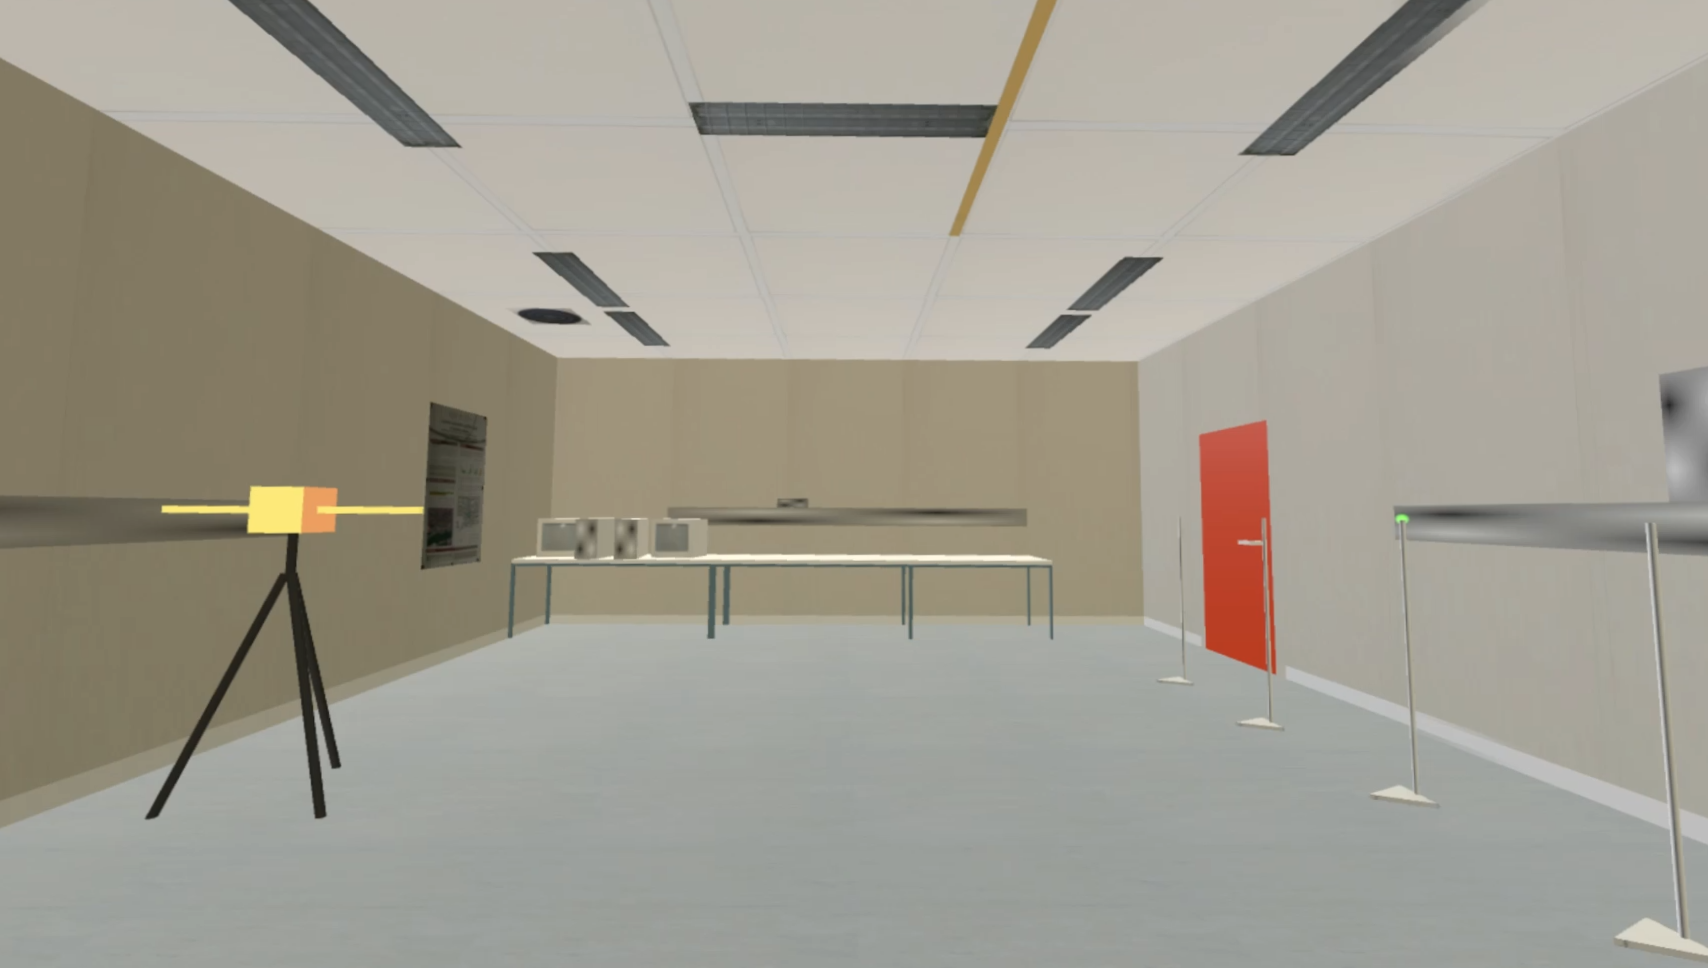
\includegraphics[width=12cm]{Images/SzenenBeispiel.png}
    \caption{Example virtual reality scene of the experiment in the light condition from the perspective of the subject.} 
    \label{SceneExampleLight}
\end{figure}
In the dark condition only the pointer and the target light were visible (see figure \ref{SceneExampleDark}). In the light condition the whole room, the pointer including its stand, the target light, and all five target-stands were visible at all times (see figure \ref{SceneExampleLight}). 
\begin{figure}
    \centering
    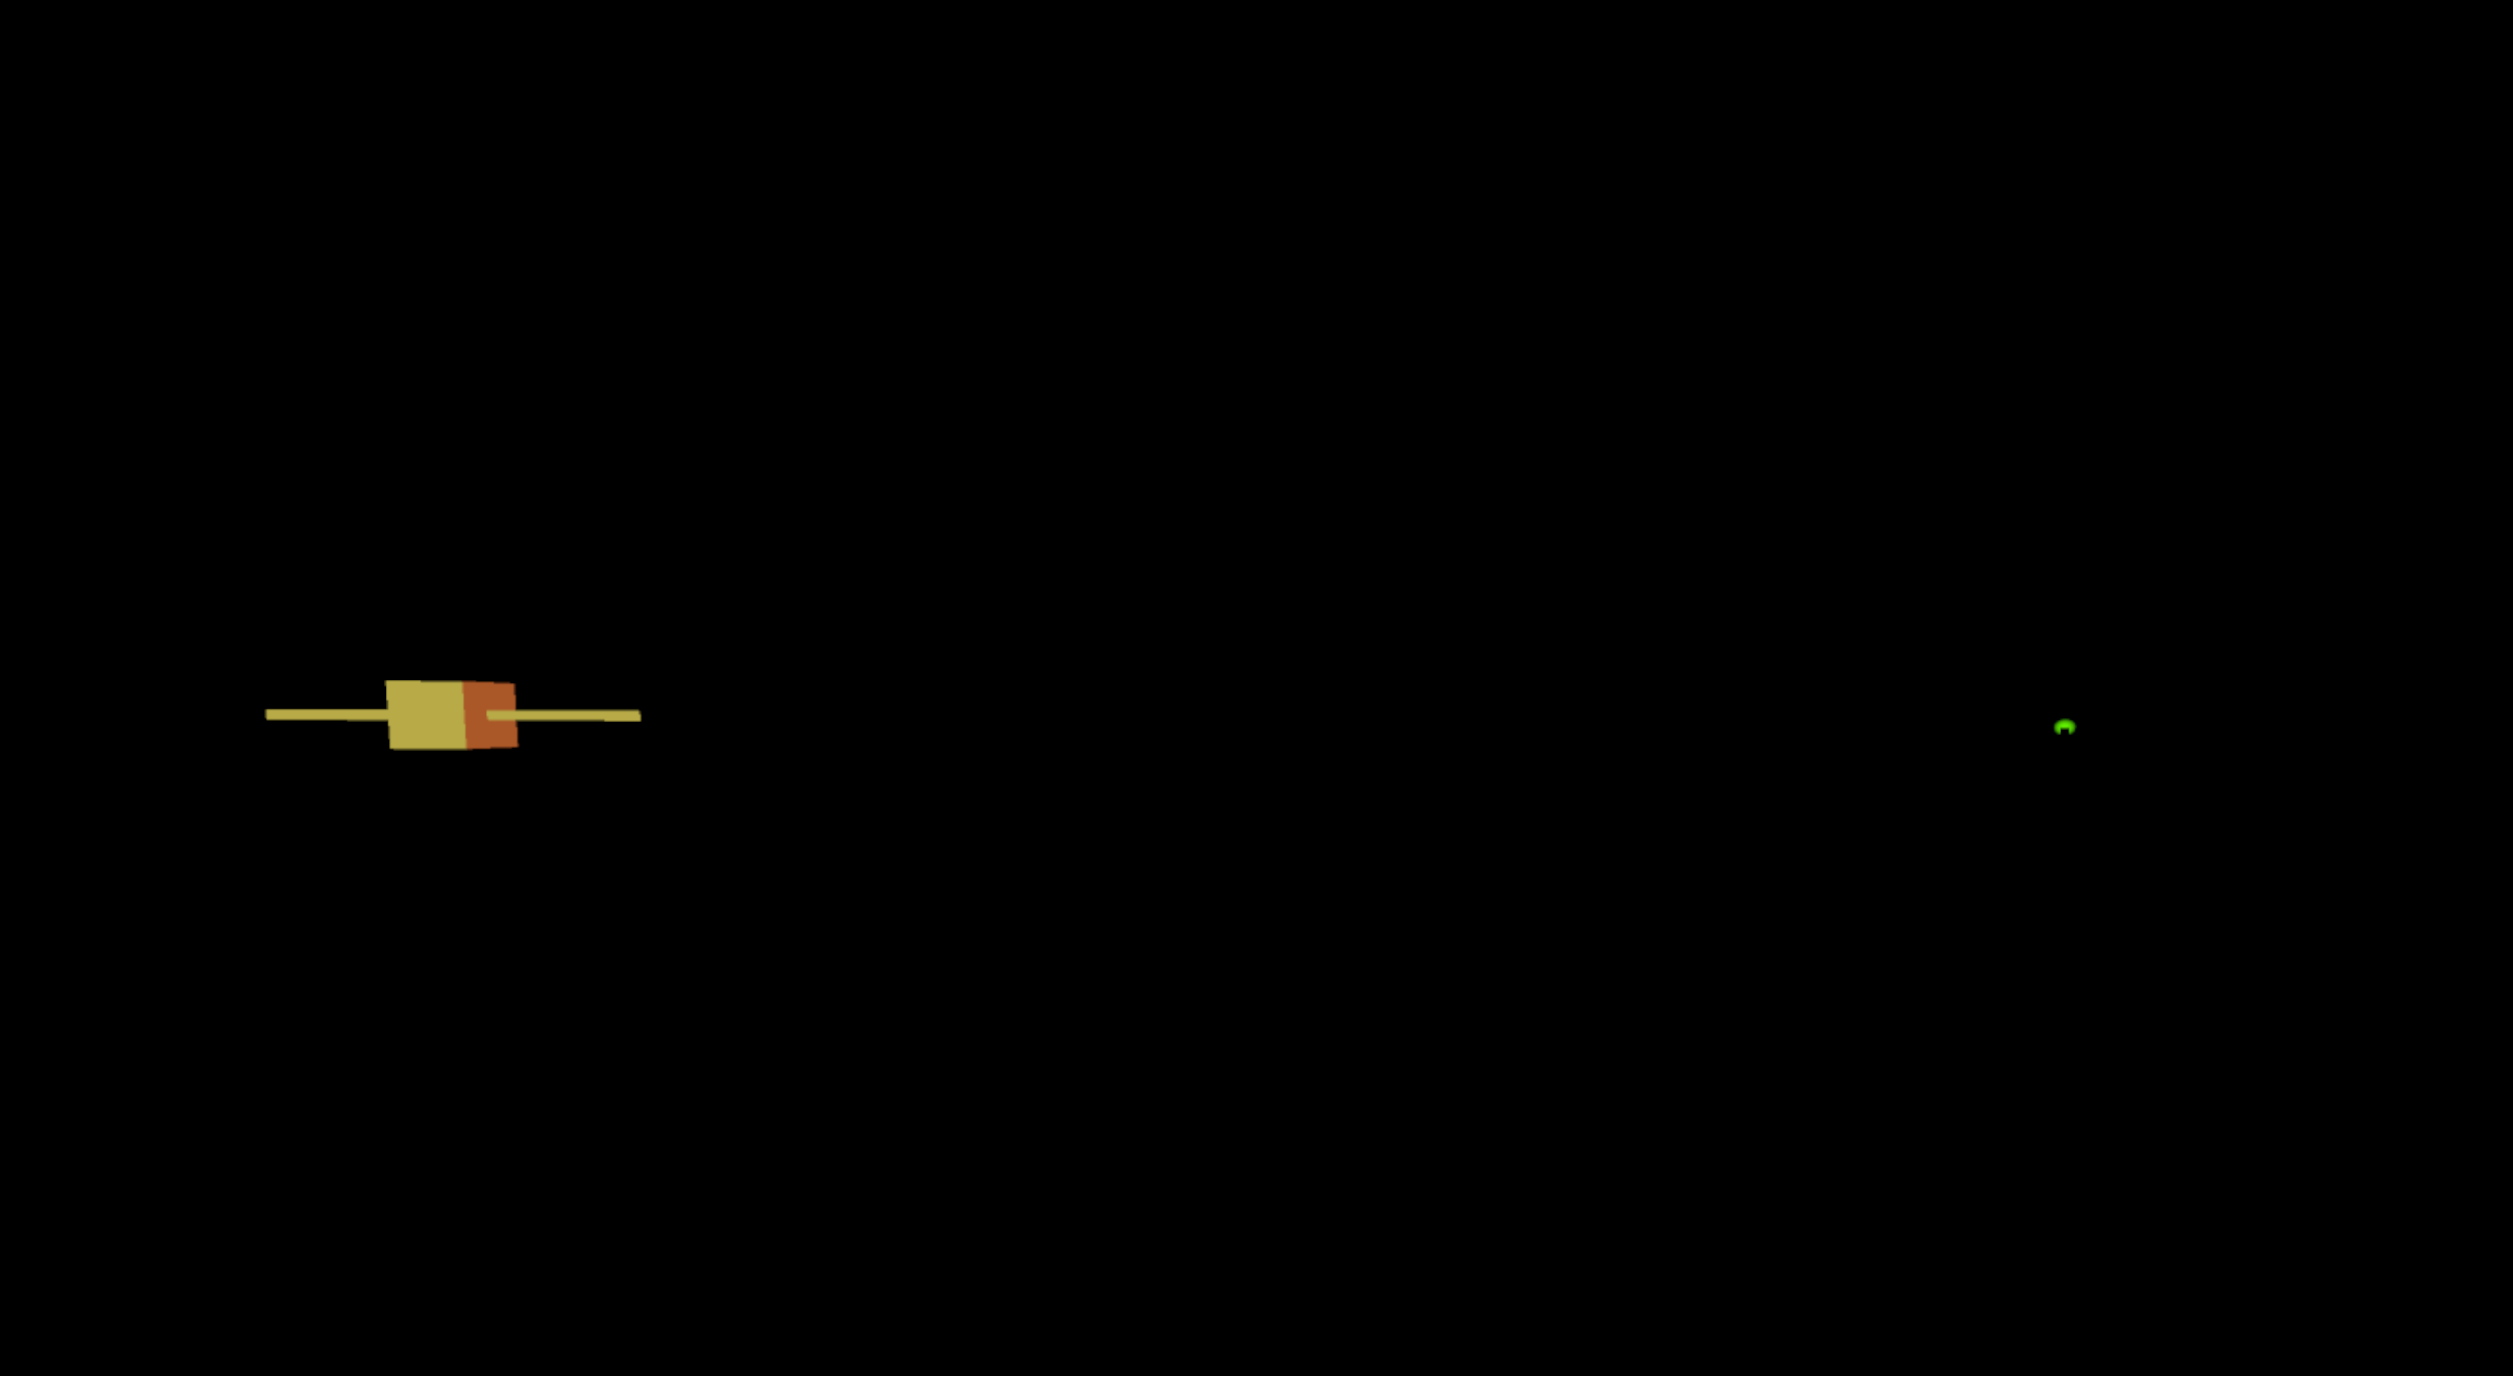
\includegraphics[width=12cm]{Images/SzeneDunkelBeispiel.png}
    \caption{Example virtual reality scene of the experiment in the dark condition, from the perspective of the subject. Note that only the pointer and the luminous target are visible.} 
    \label{SceneExampleDark}
\end{figure}

\begin{figure}
    \centering
    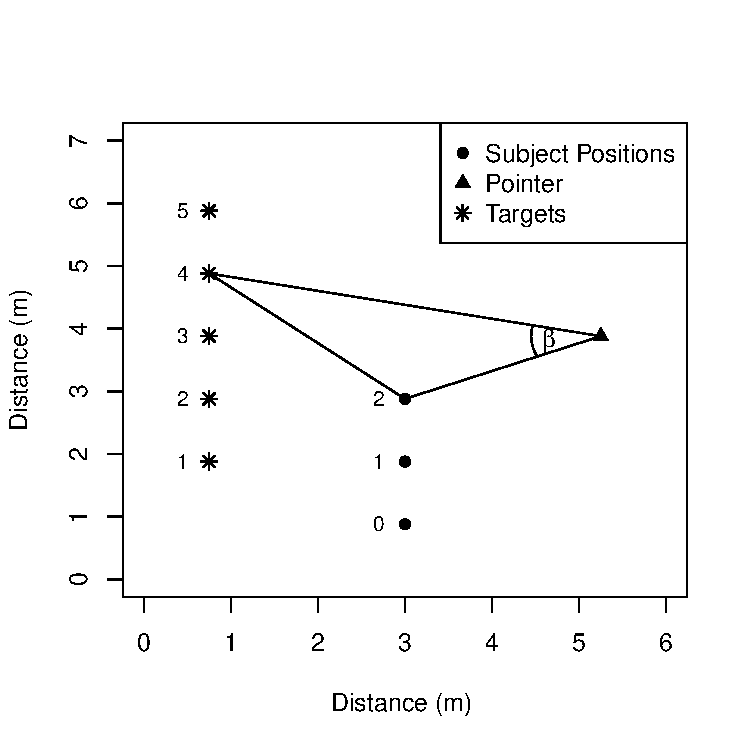
\includegraphics[width=8cm]{Images/schematicAufbau.pdf}
    \caption{Schematic image of the stimuli arrangement of the pointer right symmetry condition. Marked are the five targets, the pointer position, and the three different subject positions with $(0,0)$ marking the left rear corner of the room. Also indicated is the angle $\beta$ for one trial (subject position 2, target 4), which varied each trial depending on the target and the subject position.} 
    \label{SchematicAufbau}
\end{figure}

\section{Experimental procedure and design}
The subjects were tested in a single session of about 50 minutes ($\mu = 50.28, SD = 8.36$). Having given their informed consent, the subjects were given a controller for pointer-control, %dieser Satz ist zu lang
confirmation of set angle and pausing into their right hand and were instructed to orient the pointer towards the green light in their own time. They were able to adapt in the virtual room by some test trials (dark condition), in which they could explore the pointer control. Once they felt comfortable with handling the controller, the experiment started. In the beginning of the experiment the pointer was oriented towards the middle target stand, thus starting of in a 90\textdegree{} angle. Each trial the pointer orientation started off as it was set in the end of the preceding trial. The next trial started immediately after the subjects had confirmed the pointer's position in the preceding trial. The subjects were free to take as many breaks as they wanted. %nicht ideale überleitung zum letzten Satz


%design
The experiment was conducted as a within subject design. It consisted of 240 trials grouped into twelve blocks, in which lighting, pointer position, and subject position was varied.  Each block consisted of twenty trials, with each target-stand being targeted four times in a randomised order. The order of trials was kept the same for each block, condition and subject. The first six blocks were conducted in the dark, the later with lighting being present (dark and light condition). The experiment was symmetrically balanced with pointer and targets swapping sides after three blocks in both the dark and the light condition. In each of these blocks the subject was placed at a different position (see figure \ref{SchematicAufbau}). 

The manipulated variables were the angle $\beta$ (the angle varied between 0\textdegree{} and 77\textdegree{}) depending on the subject position and the target the subject was aiming at (see figure \ref{SchematicAufbau}), the pointer position (left or right), and the lighting (dark or light). In each frame the head rotation (x,y,z), the time stamp, and the pointer orientation angle were saved. 
%muss noch irgendwie rein:

Each of the subjects started with a different block. The first subject started at position 0 with the pointer to their left side, the second subject started at position 2 (descending subject position each block) with the pointer to their left side, the third subject at position 0 (ascending subject position each block) with the pointer to their right side, and the fourth subject started at position 2 with the pointer to their right side. All participants started with the dark condition.


% movement speed of pointer